\documentclass[journal]{IEEEtran}
\usepackage[brazil]{babel}
\usepackage[utf8]{inputenc}
\usepackage{blindtext}
\usepackage{graphicx}
\usepackage{hyperref}
\usepackage{float}
\usepackage{xcolor}

\hyphenation{op-tical net-works semi-conduc-tor}

\begin{document}
\title{Musical Genre Clustering With Self Organizing Maps}
\author{Giancarlo~Klemm}%

% Title %
\maketitle

% Abstract %
\begin{abstract}
%\boldmath
\blindtext[1]
\end{abstract}

% Key words %
\begin{IEEEkeywords}
IEEEtran, journal, \LaTeX, paper, template.
\end{IEEEkeywords}

\section{Introduction}
O clustering de músicas por gênero é um problema complexo. A extração de informações de uma música digitalizada já é extremamente complexa, mas a utilização desses dados para classificar, comparar e fazer processamentos em geral também não é uma tarefa simples. Este paper se dedica a verificar se métodos bio-inspirados geram bons resultados para calcular a similaridade entre músicas, verificando se músicas do mesmo gênero são sempre similares se comparadas com outros gêneros musicais.

O computação bio-inspirada é o uso de computadores para modelar fenômenos biológicos. Pesquisas recentes mostram que modelos bio-inspirados podem ajudar a resolver vários problemas computacionais. Um dos mais relevantes são as redes neurais, modelos que são usados para aproximar funções que dependem de um número grande de entradas e que são representados como um conjuto de neurônios interligados.

Um tipo mais específico de rede neural é o mapa de Kahonen, que tem como saída uma representação de baixa dimensão das entradas. Com um mapa de Kahonen é possível gerar um mapa de similaridade dos dados de entrada. Por isto, este método foi aplicado em um conjunto de músicas para verificar como elas são representadas e qual a relação com o seu gênero.
	
\section{Trabalho Anterior}
Os dados utilizados nestes experimentos são processados utilizando parte do programa descrito em \cite{meshup}. Este programa utiliza a biblioteca Marsyas\footnote{Marsys é uma biblioteca livre para processamento de sinais digitais. \href{http://marsyas.info/}{http://marsyas.info/}} para fazer a extração de caracteristicas de músicas digitalizadas para poder fazer comparações entre elas. Nesta implementação algumas características já foram testas para verificar quais são melhores para comparações, logo estas são usadas para fazer o cálculo de similaridade no mapa de Kahonen.

\section{Mapa de Kahonen}
De acordo com \cite{kohonen}, o mapa de Kahonen é um tipo de rede neural treinada com métodos não-supervisionados. Ela é capaz de gerar uma representação discreta de baixa dimensão para um conjunto de dados com alta dimensão. Nesta publicação os dados com alta dimensão são as caracteristicas extraídas de músicas digitalizadas, enquanto que a saída é um gráfico 2D representando a semelhança entre cada elemento.

Como em uma rede neural convencional, um mapa de Kahonen formado por vários neurônios interligados, sendo que certos neurônios recebem as entradas e propagam a informação para outros neurônios até que um neurônio de saída seja ativado. A diferença de um mapa de Kahonen é que ele é treinado usando Competitive Learning\footnote{Normalmente uma rede neural é treinada utilizando métodos de correção de erros como propagação para trás ou método gradiente.}.

\textit{Competitive Learning}~\cite{c-learning} é um método de treinamento não-supervisionado onde neurônios competem pelo direito de representação um subconjunto dos dados da entrada. Ou seja, as propriedades topológicas dos dados de entrada são preservadas. Este método funciona aumentando a especialização em cada neurônio da rede, fazendo com que seja ideal para clustering.

\section{Conjunto de dados}
O conjunto de dados utilizado é a coleção de músicas Marsyas GTZAN (\href{https://github.com/JustGlowing/minisom}{https://github.com/JustGlowing/minisom}). Este conjunto foi coletado de 2000-2001 de diversas fontes e contêm 1000 segmentos de 30 segundos cada. Há 10 gêneros diferentes com 100 músicas para gênero.

\section{Extração das caracteristicas}
As caracteristicas das músicas foram extraídas utilizando técnicas de processamento de sínais digitais encontradas na biblioteca Marsyas. As seguintes caracteristicas foram extraídas:
\begin{itemize}
	\item Andamento: É o grau de velocidade da música. Apesar de variar muito mesmo entre músicas do mesmo gênero, a comparação do andamento de um conjunto de dados pode diferenciar gêneros parecidos (Exemplo: Diferenciar o rock clássico do rock pesado).
	\item Tom: Se refere a nota em relação à qual se constrói as escalas da música. Este elemento tende a ser bom para comparações pois músicas do mesmo gênero tendem a usar as mesmas escalas ou escalas parecidas (Exemplo: Escala pentatonica no gênero Blues).
	\item Tempo: É a pulsação básica subjacente de uma composição qualquer. Não se deve confundir tempo com andamento, onde tempo é refente ao "tempo musical" e o andamento é refente ao "tempo real".
	\item Timbre médio: O timbre é a qualidade de uma nota músical que difere tipos de produções de som. Está relacionado com a fonte/instrumento da música.
	\item Média e desvío padrão dos MFCCs (Mel-frequency Cepstral Coefficients): São coeficientes para representação do som baseado na percepção auditiva humana. Eles são derivados a partir de transaformadas inversas de fourier, aplicada nas janelas de frequências da música.
\end{itemize}

\section{Implementação do mapa de Kahonen}
A implementação utilizada para o mapa de Kohenen foi a Minisom, que pode ser encontrada em \href{https://github.com/JustGlowing/minisom}{https://github.com/JustGlowing/minisom}. Sobre essa implementação:
\begin{center}
``Minisom é uma implementação minimalista baseada em Numpy de um mapa de Kahonen. Um mapa de Kahonen é um tipo de rede neural capaz de converter relações complexas não-lineares entre itens em relaçoes geométricas simples.''
\end{center}

\section{Metodologia}
Para os testes, redes de tamanho 7x7 até 15x15 foram utilizadas. Com $\sigma=3.0$, taxa de aprendizagem 0.5 e com método de treinamento aleatório usando 100 iterações.

Os gêneros utilizados para os testes foram:
\begin{itemize}
	\item Clássico
	\item Eletrônico
	\item Folk
	\item Rock Clássico
	\item Reggae
\end{itemize}

Para cada gênero, 100 músicas foram utilizadas. Vários testes foram feitos usando permutações diferentes das características disponíveis e gêneros musicais para fazer uma análise sobre quais caracteristicas são melhores para o conjunto de dados utilizados.

\section{Resultados}
\subsection{Andamento, Tom e Tempo}
Os primeiros testes feitos utilizaram as características mais teóricas das músicas- Andamento, Tom e Tempo - por terem relações fortes entre sí.

\begin{figure}[H]
\centering
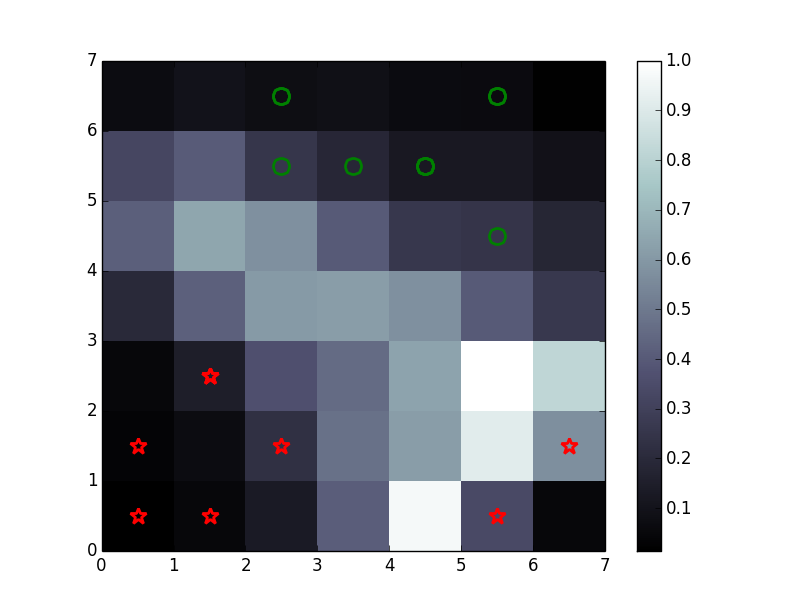
\includegraphics[scale=0.5]{images/key_tempo_rock_eletronic.png}
\caption{Rock em \textcolor{red}{Vermelho}, Eletrônico em \textcolor{green}{Verde}.}\label{key_tempo_rock_eletronic}
\end{figure}

A figura \ref{key_tempo_rock_eletronic} mostra o mapa da comparação entre os gêneros Rock e Eletrônico. É possível ver uma clara divisão entre os gêneros, apesar de haver um certa divisão dentro do gênero Rock. Isso é mais acentuado no resultado da comparação entre Rock e Folk na figura \ref{key_tempo_rock_folk}.

\begin{figure}[H]
\centering
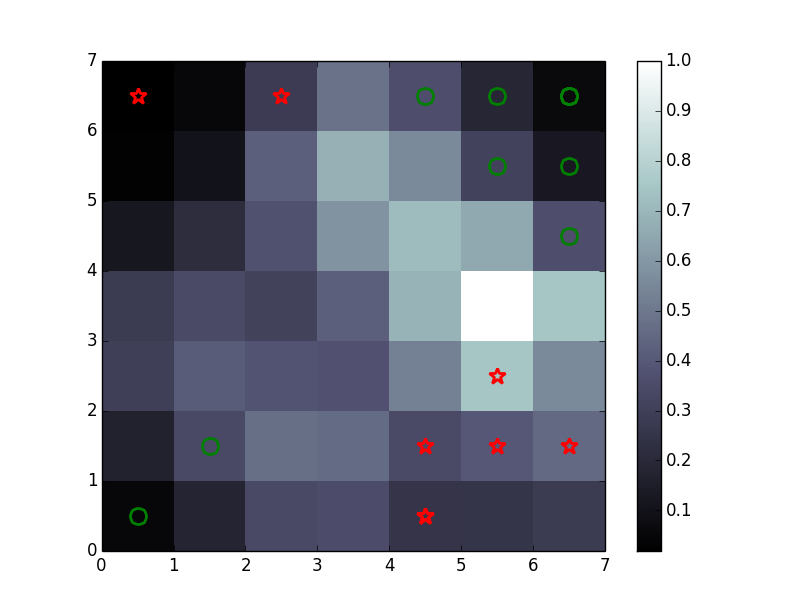
\includegraphics[scale=0.5]{images/key_tempo_rock_folk.png}
\caption{Rock em \textcolor{red}{Vermelho}, Folk em \textcolor{green}{Verde}.}\label{key_tempo_rock_folk}
\end{figure}

Isso acontece quando a diferença com relação as caracteristicas de cada grupo é muito pequena. Logo, qualquer pequena difença acaba gerando um novo grupo de neurônios. É possível identificar isso nos resultados pois Rock e Folk são muito mais parecidos que Rock e Eletrônico, logo a divisão é menos precisa.

Nas figuras \ref{key_tempo_rock_reggae} e \ref{key_tempo_rock_classical_folk} temos divisões mais precisas. No caso do Rock e do Reggae, as caracteristicas são bem distintias entre os grupos, e caso do Clássico, Rock e Folk a diferença não é tão grande entre os dois grupos Rock e Fol), mas é com relação ao Clássico.

\begin{figure}[H]
\centering
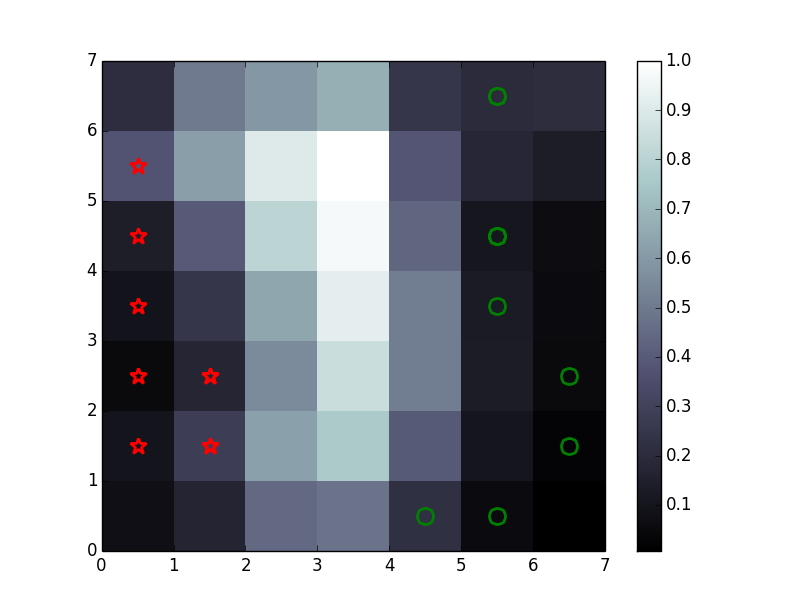
\includegraphics[scale=0.5]{images/key_tempo_rock_reggae.png}
\caption{Rock em \textcolor{red}{Vermelho}, Reggae em \textcolor{green}{Verde}.}\label{key_tempo_rock_reggae}
\end{figure}

\begin{figure}[H]
\centering
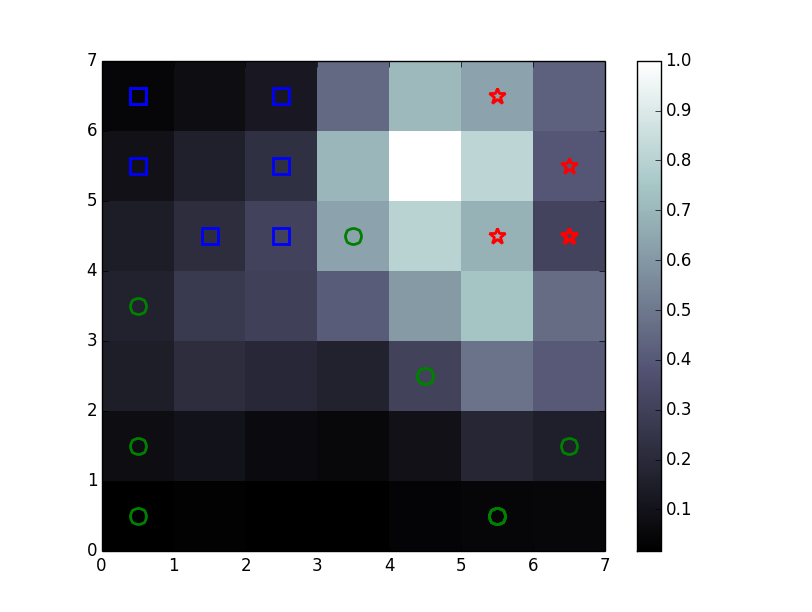
\includegraphics[scale=0.5]{images/key_tempo_rock_classical_folk.png}
\caption{Clássico em \textcolor{red}{Vermelho}, Rock em \textcolor{green}{Verde}, Folk em \textcolor{blue}{Azul}.}\label{key_tempo_rock_classical_folk}
\end{figure}

Apesar de nos casos anteriores as divisões serem razoavelmente visíveis para essas caracteristicas, há casos em que elas não funcionam bem (Figura \ref{key_tempo_classical_eletronic_folk}). Parte das músicas do gênero Clássico estão no cluster do gênero Eletrônico, e sonoramente as músicas são muito distintas. Isso ocorre pois as caracteristicas não estão representado bem este conjunto de músicas.

\begin{figure}[H]
\centering
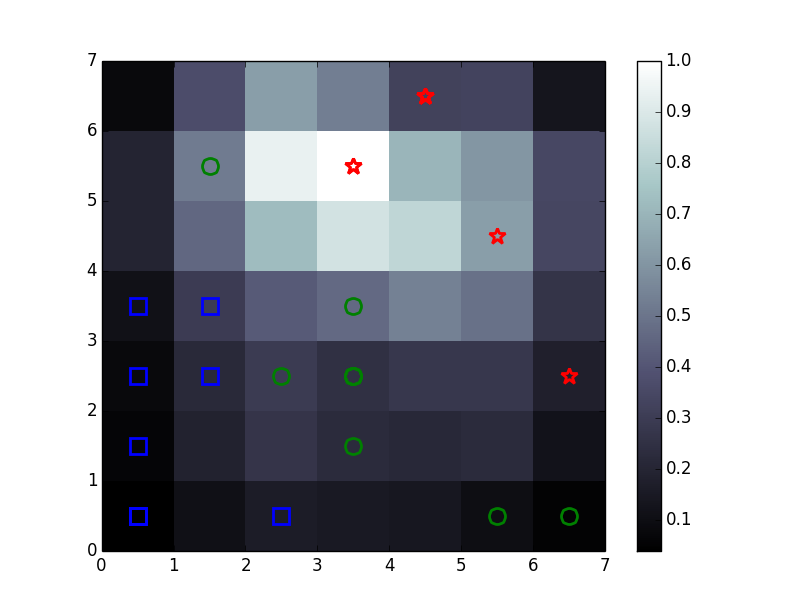
\includegraphics[scale=0.5]{images/key_tempo_classical_eletronic_folk.png}
\caption{Folk em \textcolor{red}{Vermelho}, Clássico em \textcolor{green}{Verde}, Eletrônico em \textcolor{blue}{Azul}.}\label{key_tempo_classical_eletronic_folk}
\end{figure}

\subsection{Timbre}
As figuras \ref{timbre_rock_folk_classical} e \ref{timbre_classical_reggae_eletronic} mostram os resultados do mapa de comparações utilizando o timbre extraído das músicas. Os resultados para a comparação entre Rock, Clássico e Folk é parecido com quando foi utilizado o andamento, tom e e tempo. Porém na comparação entre Clássico, Folk e Eletrônico a divisão é bem imprecisa, com geração de vários péquenos grupos.

\begin{figure}[H]
\centering
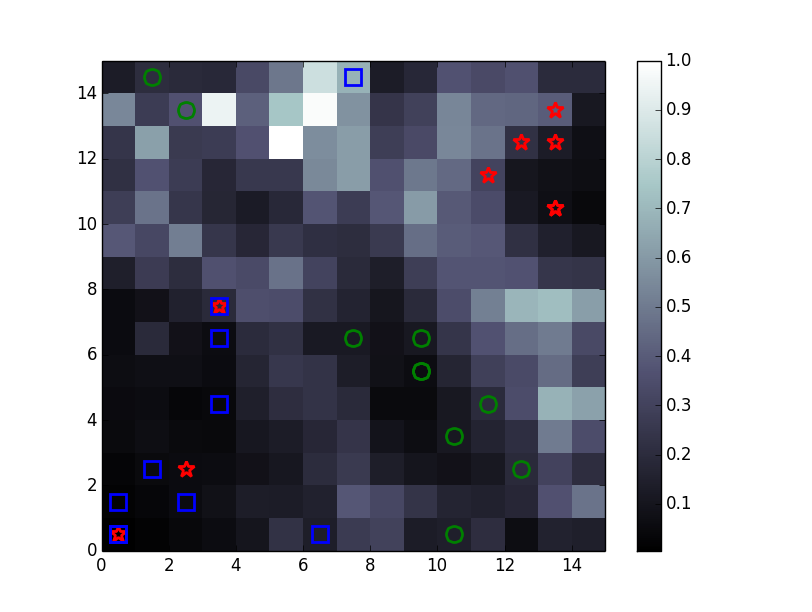
\includegraphics[scale=0.5]{images/timbre_rock_folk_classical.png}
\caption{Rock em \textcolor{red}{Vermelho}, Clássico em \textcolor{green}{Verde}, Folk em \textcolor{blue}{Azul}.}\label{timbre_rock_folk_classical}
\end{figure}

\begin{figure}[H]
\centering
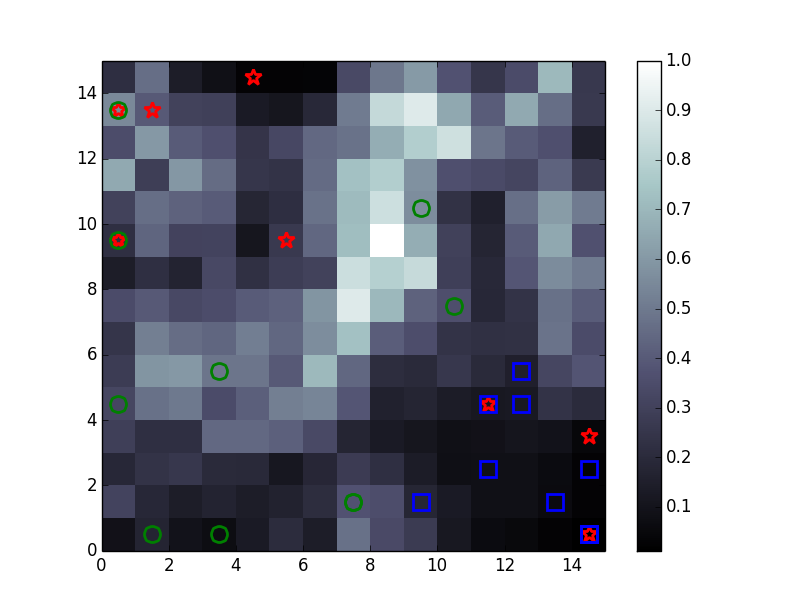
\includegraphics[scale=0.5]{images/timbre_classical_reggae_eletronic.png}
\caption{Clássico em \textcolor{red}{Vermelho}, Folk em \textcolor{green}{Verde}, Eletrônico em \textcolor{blue}{Azul}.}\label{timbre_classical_reggae_eletronic}
\end{figure}

No geral, o timbre se mostrou uma caracteristica inconsistente, principalmente com comparações entre gêneros que utilizam instrumentos musicais mais variados. Parte do problema com o uso do timbre se deve a etapa de extração do timbre como caracteristica, pos é uma das informações que mais se perdem durante a transformação de físico para digital (Gravação de uma música).

\subsection{MFCCs}
As comparações feitas utilizando MFCCs como caracteristicas de similaridade resultam em grupo bem definidos, com diferenciações precisas entre os gêneros musicais (Figuras \ref{mfccs_rock_classical_eletronic}, \ref{mfccs_rock_reggae_folk} e\ref{mfccs_classical_eletronic}). Como o MFCC se baseiam na frequência, as diferenças são mais marcantes, inclusive com gêneros parecidos como Rock e Folk.
É possível dizer que os MFCCs fazem uma divisão melhor pois eles não utilizam informações separadamente. Ao contrário, a frequência é afetada por todas as outras caracteristicas citadas.

\begin{figure}[H]
\centering
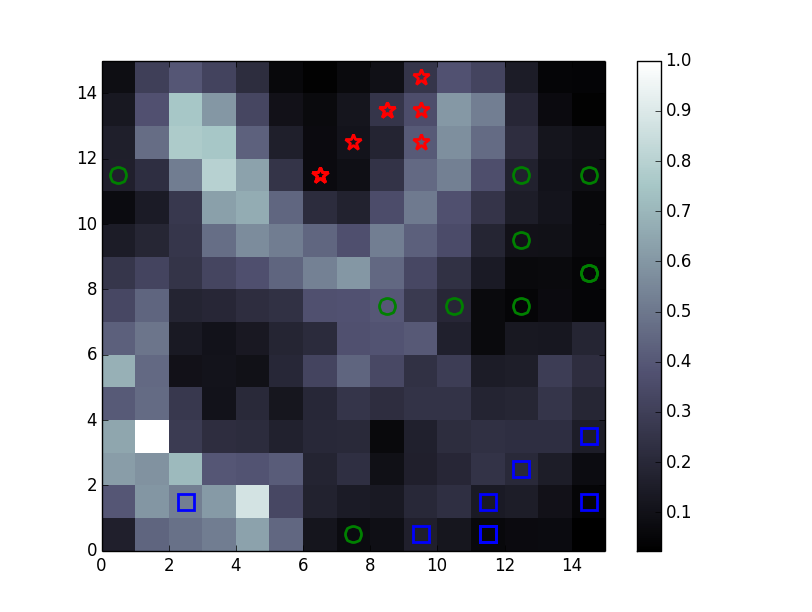
\includegraphics[scale=0.5]{images/mfccs_rock_reggae_folk.png}
\caption{Rock em \textcolor{red}{Vermelho}, Reggae em \textcolor{green}{Verde}, Folk em \textcolor{blue}{Azul}.}\label{mfccs_rock_reggae_folk}
\end{figure}

\begin{figure}[H]
\centering
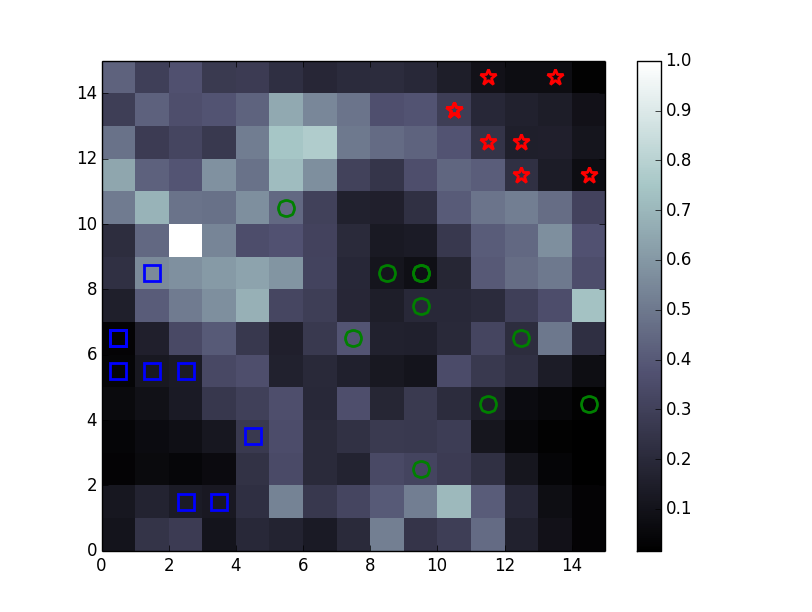
\includegraphics[scale=0.5]{images/mfccs_rock_classical_eletronic.png}
\caption{Rock em \textcolor{red}{Vermelho}, Clássico em \textcolor{green}{Verde}, Eletrônico em \textcolor{blue}{Azul}.}\label{mfccs_rock_classical_eletronic}
\end{figure}

\begin{figure}[H]
\centering
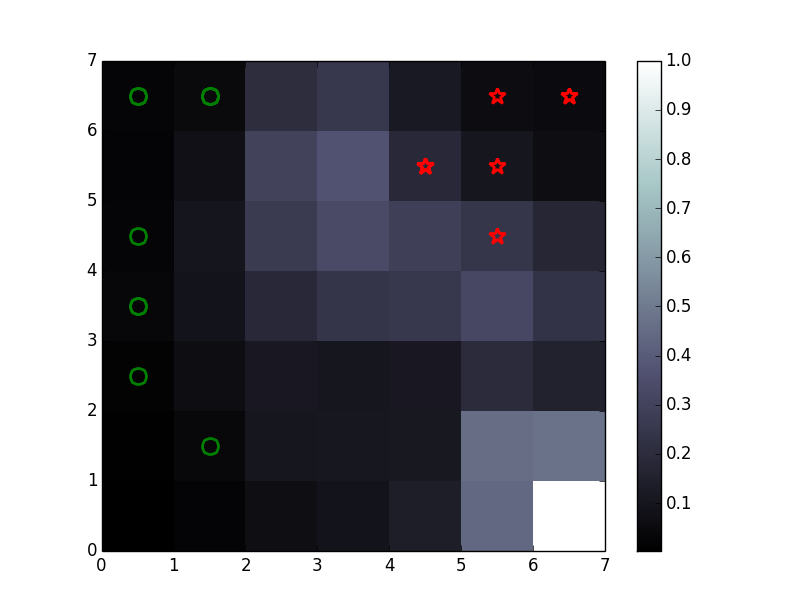
\includegraphics[scale=0.5]{images/mfccs_classical_eletronic.png}
\caption{Clássico em \textcolor{red}{Vermelho}, Eletrônico em \textcolor{green}{Verde}.}\label{mfccs_classical_eletronic}
\end{figure}

\section{Conclusão}
O uso do mapa de Kohonen para clustering de músicas com relação a seus gêneros se provou razoavelmente eficiente, gerando grupos bem definidos na maioria dos casos.

Mais especificamente, os MFCCs se mostraram as melhores caracteristicas para essa comparação de similaridade. O conjunto de caracteristicas Tempo, Andamento e Tom também teve bons resultados, embora um pouco menos precisos. A utilização destes em conjunto com os MFCCs (Com maior peso para os MFCCs) tem resultados ainda mais precisos. Pelo resultado dos experimentos é possível ver que o timbre não é uma boa caracteristica para se comparar gêneros musicais, resultando em mapas com divisão pouco precisa.


\ifCLASSOPTIONcaptionsoff
  \newpage
\fi

\begin{thebibliography}{1}

\bibitem{kohonen}
Teuvo Kohonen \emph{Self-Organized Formation of Topologically Correct Feature Maps}, Biological Cybernetics 43 (1): 59–69, 1982.

\bibitem{c-learning}
David Rumelhart, David Zipser, James L. McClelland \emph{Parallel Distributed Processing}, Vol. 1. MIT Press. pp. 151–193, 1986.
  
\bibitem{meshup}
G.~Klemm, R.~Valle, T.~Lima, \emph{Automatic Support for Digital Mashups}, 2014. \href{https://github.com/giancarlokc/Automated-Mesh-up/blob/master/paper.pdf}{https://github.com/giancarlokc/Automated-Mesh-up/blob/master/paper.pdf}. 

\end{thebibliography}

\end{document}


